\chapter{Estado da Arte}\label{cap:estArte}

%\lipsum[34]

No presente capítulo serão apontados os fundamentos teóricos nos quais o desenvolvimento do sistema web de gerenciamento foram embasados, ou seja, como se constituem os padrões de organização do RoR e o comportamento de aplicações web. Adicionalmente, mostra-se uma descrição cuidadosa e sucinta de trabalhos relacionados à área do sistema desenvolvido, que mostram um recorte adequado para visualização do universo de estudo. Em seguida, apresentam-se os atores, isso é, os usuários finais do sistema. Como mencionado anteriormente, o software é direcionado à comunidade acadêmica do IFRN. Também são apresentadas, detalhadamente, todas as funcionalidades e delimitações do software. Na última seção, serão mostrados o diagrama de casos e uso. Uma perspectiva comparativa será realizada, relacionando as possibilidades possíveis de cadastramento .  

\section{Desenvolvimento web}%\label{sec:primTrab}
%\addcontentsline{toc}{section}{Desenvolvimento web}

Desenvolvimento web é o termo utilizado para descrever a criação de sites, na Internet ou numa intranet. Atualmente, alguns sites são aplicativos complexos capazes de 
realizar transações, apresentar dados em tempo real,
e fornecer experiências interativas ao usuário. Os software baseados na web estão se tornando tão poderosos e importante quanto
software de mesa. A grande maioria dos aplicativos da web produzidos fornecem funcionalidades avançadas, e isso é uma tarefa complexa que envolve um considerável número de conjuntos de ferramentas, e muitas opções. As estruturas da web criadas com tais tecnologias necessitam de um gerenciamento de conteúdo. Para esse objetivo, costuma-se utilizar ferramentas que construam uma estrutura web, permitindo escolher entre diferentes tipos de elementos que melhor atendam as necessidades \cite{HackerScot2008}.
Em sua investigação, \cite{plekhanova2009evaluating}, avaliou  três estruturas de desenvolvimento web principais de código fonte abertas: Django, Ruby on Rails (RoR) e CakePHP, escritos em três linguagens diferentes - Python, Ruby e PHP, respectivamente. Todas as três estruturas citadas têm arquiteturas semelhantes e reivindicam ter características parecidas, como produtividade aprimorada e reutilização de código. Em sua conclusão, a autora classificou as ferramentas segundo critérios
que verificaram:
\begin{itemize}
	\item Os componentes front-end e back-end (desenvolvimento da interface do usuário, gerenciamento e migração de dados).
	\item O desempenho total
	 das estruturas (manutenibilidade, testabilidade).
	 \item A popularidade, difusão na comunidade, maturidade e comercialização.
\end{itemize}

A conclusão geral dessa autora foi de que todas as três estruturas são ferramentas robustas e a escolha qual utilizar precisa considerar o contexto de aplicação. As empresas e os profissionais de desenvolvimento web necessitam individualizar o processo avaliativo de escolha ao seu contexto único.


\nocite{an2009static}

\cite{lei2014performance}, realizou uma investigação concentrando-se no impacto do desempenho de três diferentes tecnologias da Web: Node.js, PHP e
Python-Web. No entanto, negligenciou os problemas de segurança e escalabilidade. Nessa perspectiva, desenvolveu um método universal de avaliação da técnica de desenvolvimento web com base na comparação do desempenho das ferramentas analisadas. Em sua conclusão verificou que o Node.js tem um desempenho muito melhor que o tradicional PHP em situação de alta simultaneidade e que o Python-Web também não é adequado para o uso intensivo em computação. 

Em síntese, pode-se argumentar que o gerenciamento de conteúdo da web é o resultado da entrega de material para a web. O crescimento do número de páginas da web tornou-se popular nas últimas décadas  e os padrões Model-View-Controller (MVC) facilitaram bastante seu desenvolvimento \cite{mckeever2003understanding}. Eles ocultam a complexidade, dão estrutura e consistência e promovem as melhores práticas.

A partir de sua experiência, \cite{tapiador2012content}  explora a criação de sistemas de gerenciamento de conteúdo da web com
Ruby on Rails, uma estrutura popular de desenvolvimento web produzida para aumentar a produtividade. Em sua investigação o autor explica as vantagens da implementação
da arquitetura MVC baseando-se nos príncipios de “convention over configuration” (convenção sobre configuração) e “don’t repeat yourself” (não se repita) \cite{bachle2007ruby}.

Diante dessa realidade, no presente trabalho de conclusão de curso, optou-se, como componente orientador do processo de desenvolvimento do sistema de gerenciamento de estacionamentos, aderir à doutrina Rails \cite{taylor2010rails}, uma vez que partindo desta ferramenta é possível estabelecer as consistências e as principais
dependências do sistema \cite{astels2002extreme}.

\section{Descrição da arquitetura Model-View-Controller}

O Rails possiu diversas características interessantes. Dessa propriedades, pode-se destacar algumas considerações bastante sérias, por exemplo as restrições sobre como se estrutura a construção dos aplicativos da web. Surpreendentemente, essas restrições, na realidade, facilitam a criação dos aplicativos.
Elaborado em 1979 por Trygve Reenskaug, essa forma de organização é aplicada no desenvolvimento de funcionalidades interativas, dividindo-se em modelos, visões e controladores \cite{ruby2009agile}. 
O modelo é responsável por manter o estado do aplicativo. As vezes
esse estado é transitório, durando apenas algumas interações com o usuário. Às vezes, o estado é permanente e é armazenado fora do aplicativo, frequentemente em um banco de dados.


A visualização é responsável por gerar uma interface com o usuário, normalmente baseados em dados do modelo. Embora a visualização possa apresentar ao usuário
várias maneiras de inserir dados, a própria exibição nunca lida com dados recebidos.
O trabalho da visualização é concluído depois que os dados são exibidos. 
Os controladores recebem eventos do
mundo exterior (normalmente, a entrada de utilizador), interagem com o modelo, e apresentam uma pespectiva apropriada para o usuário.
Na atualidade, o padrão de organização MVC prevalece como aspecto de criação dos frameworks. 


Em geral, os aplicativos da web guardam suas informações em um banco de dados relacional. Os sistemas de entrada de solicitações armazenam informações e detalhes do cliente em tabelas de banco de dados. As consultas ao banco de dados relacionais são fundamentadas matematicamente na  teoria de conjuntos. Porém, existe uma certa dificuldade em combinar bancos de dados relacionais com linguagens de programação orientadas a objetos (OO).
Os objetos lidam com dados e operações, e os bancos de dados são todos sobre conjuntos de valores. Muitas vezes, torna-se complicado expressar termos relacionais  codificando-os em um sistema OO. O contrário também é verdade. 

\begin{figure}[h]
	\caption{Estrutura MVC do RoR.}
	
	\centering % para centralizarmos a figura
	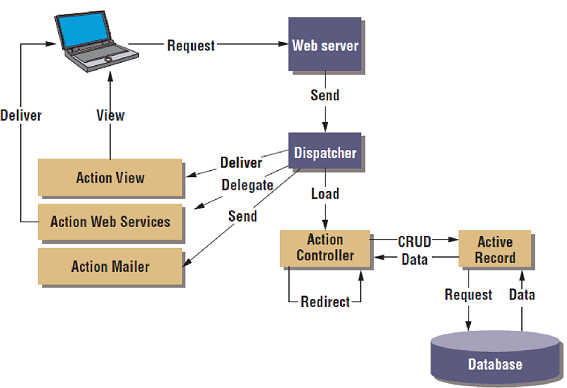
\includegraphics{Figs/frameworkRuby.png} % leia abaixo
	\label{figura:frameworkRuby}
\end{figure}
%Na seção seguinte será apresentada a maneira particular como o Rails realiza o mapeamento dos dados relacionais em objetos.
%Amparado nesta realidade, o presente trabalho, foi realizado utilizando a ferramenta Ruby on Rails. Nos próximos capítulos....

Na seção seguinte serão apresentados os atores, requisitos funcionais e não funcionais, o diagrama de caso de uso e informações sobre o banco de dados utilizado.

\section{Requesitos do Sistema}
\subsection{Ator}
Os atores que poderão acessar o sistema são os seguintes:
 
 \textbf{Porteiro:} É o funcionário do IFRN responsável por realizar o cadastramento dos demais servidores ou alunos.
 
 \textbf{Administrador:} É o funcionário do setor de TI responsável pela administração da plataforma. Esse ator tem as permissões necessárias para gerenciar a plataforma, realizando atualizações e melhorias, se necessárias.
 \subsection{ Requisitos Funcionais}
 
 Na descrição desse tópico serão descritas as aplicações dos usuários definidos anteriormente.
As ações dos atores estão relacionadas aos requisitos estabelecidos pelo sistema \cite{SOMMERVILLE}, \cite{pressman2016engenharia}.\\\\\\1º Requisito Funcional\\
 \textbf{Cadastro de Usuários:} No software desenvolvido é utilizada a \texttt{gem} 'devise'  para cadastrar novos usuários.\\
 2º Requisito Funcional\\
 \textbf{Autenticação:}  A  \texttt{gem} 'devise' proporciona ao software a geração de uma tela de login onde o usuário
 informa suas habilitações obtendo acesso à plataforma de gerenciamento.
 3º Requisito Funcional\\
 \textbf{Redefinição de Senha:} A  \texttt{gem} 'devise' prepara a página de cadastramento de maneira que possa  enviar um link para o e-
 -mail do usuário para redefinição de senha, caso seja solicitada.\\
  4º Requisito Funcional\\
 \textbf{Cadastramento do estacionamento:}
 A  \texttt{gem} 'Admin' permite a geração de modelos sem a necessidade da criação de \textit{Controller} ou rotas. Dessa maneira, gerou-se os demais modelos, a saber, modelos para o cadastramento de: \textbf{veículo},
  %6º Requisito Funcional\\
 \textbf{tipo de vaga} e
  %7º Requisito Funcional\\
 \textbf{funcionário}.\\
 5º Requisito Funcional\\
 \textbf{Edição dos cadastros:}  A  \texttt{gem} 'Admin' prepara automaticamente a possibilidade de edição dos cadastros realizados. Nesse caso é possível atualizar, remover e exportar.
 
 \subsection{Requisitos Não-Funcionais}
 Define-se requisitos não-funcionais como aqueles que não possuem relacionamento direto com
 as atividades do software. Porém, são limitações dos serviços oferecidos pelo
 software \cite{rezende2006engenharia}.\\
 1º Requisito Não-Funcional\\
 \textbf{Incompatibilidade com dispositivos móveis:}
 O software não é compatível com dispositivos móveis.\\
 2º Requisito Não-Funcional\\
 \textbf{Acessos Simultâneos:}
 O banco de dados \texttt{postgresql} não possui limitação. No entanto, para proteção de acessos simultâneos, configurou-se um limite, restrito a uma faixa de IPs. Caso seja necessário uma maior capacidade, existe a possibilidade de modificação.
 
 \section{Diagrama de Casos de Uso}
 
 
 
 \begin{figure}[h]
 	\caption{Diagrama de Caso de Uso}
 	%\flushright
 	\centering % para centralizarmos a figura
 	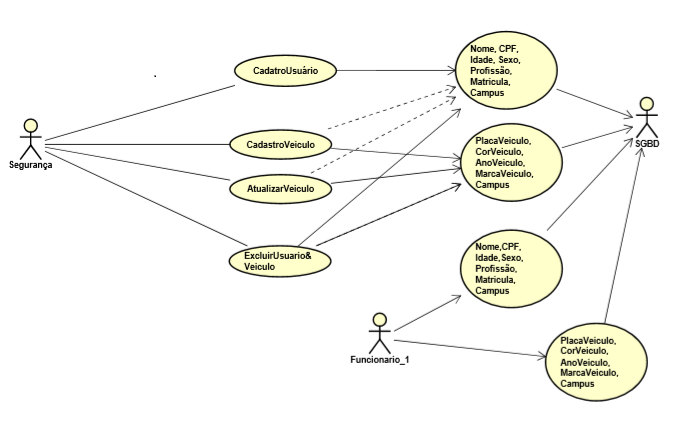
\includegraphics{Figs/diagramaCasoUso_proj_vic.png} % leia abaixo
 	\label{figura:diagramaCasoUso_proj_vic}
 \end{figure}
 
%\lipsum[34-36]